% Set the encoding before IEEEtran initializes its Times font metrics.
\RequirePackage[T1]{fontenc}
\documentclass[conference]{IEEEtran}
\IEEEoverridecommandlockouts

% Keep the submission geometry explicit and compatible with the IEEE template.
\pdfpagewidth=8.5in
\pdfpageheight=11in

\usepackage{cite}
\usepackage{amsmath,amssymb,amsfonts}
\usepackage{amsthm}
\usepackage{graphicx}
\usepackage{array}
\usepackage{booktabs}
\usepackage{textcomp}
\usepackage{xcolor}
\usepackage[hyphens]{url}

% Keep the conference layout dense enough for a systems-paper draft while
% preserving IEEEtran's type sizes and margins.  The manuscript contains many
% small analytical figures and tables; reducing float whitespace makes their
% relationships visible without shrinking the body text.
\setlength{\textfloatsep}{5pt plus 1pt minus 2pt}
\setlength{\floatsep}{4pt plus 1pt minus 2pt}
\setlength{\intextsep}{5pt plus 1pt minus 2pt}
\setlength{\abovecaptionskip}{2pt}
\setlength{\belowcaptionskip}{0pt}
\setlength{\tabcolsep}{3pt}

% APPT's original vector figures use PDF 1.7. Keep the container compatible
% with both pdfLaTeX and the XeTeX/xdvipdfmx backend used by Tectonic.
\ifdefined\pdfminorversion
  \pdfminorversion=7
\else
  \AtBeginDocument{\special{pdf:minorversion 7}}
\fi

\newcommand{\system}{\textsc{cuButterfly}}
\newcommand{\pending}[1]{\textcolor{gray}{[Pending: #1]}}
\newcommand{\CurrentFFTSingle}{1.298}
\newcommand{\CurrentFFTDouble}{1.366}
\newcommand{\CurrentNTT}{1.188}
\newcommand{\CurrentFWHT}{1.474}
\newcommand{\CurrentCyclicNTT}{1.308}
\newcommand{\CurrentCKKSLoop}{1.428}
\newcommand{\CurrentCKKSBatch}{1.218}
\newcommand{\CurrentCKKSFast}{1.131}


% Internal layout examples are excluded by the evidence-only wrapper.
% Synthetic numbers must never become evidence by removing their watermark.
\newif\ifdraftfigures
\ifdefined\cBNoDraftFigures
  \draftfiguresfalse
\else
  \draftfigurestrue
\fi

\newtheorem{proposition}{Proposition}
\newcounter{boundaryalgorithm}

\def\BibTeX{{\rm B\kern-.05em{\sc i\kern-.025em b}\kern-.08em
    T\kern-.1667em\lower.7ex\hbox{E}\kern-.125emX}}

\begin{document}
\pagenumbering{arabic}

\title{cuButterfly: Unleashing Performance of Butterfly Computation with Hybrid Tile Dataflow Graph}
\author{\normalsize{ISCA 2026 Internal Working Draft -- Anonymous -- Do Not Distribute}}

\maketitle
\thispagestyle{plain}
\pagestyle{plain}

\begin{abstract}
Butterfly computation underlies Fourier, number-theoretic, Hadamard, and zeta
transforms. Their arithmetic differs, yet their implementations face a common
problem of organizing staged dependencies under finite storage and parallel
resources. We present \system{}, a dependency-derived execution framework for
these computations. Ordered stage bits identify \emph{dependency-closed
subgraphs} and their communication. \emph{Hierarchical hybrid dataflow}
combines local residency with streamed execution across storage scopes, while
\emph{successor-aligned writeback} constructs compatible boundary layouts.
Operator semantics, workload domains, and hardware capabilities specialize
this shared construction. Compatible arithmetic cores and measured services
guide generation and bounded search.

A bounded A100 80GB operator screen observes geometric-mean latency ratios
of 1.103$\times$ and 1.353$\times$ over cuFFT for its FP32 and FP64 requests.
A separate exact-checked NTT batch study reaches 1.285$\times$ over GPU-NTT.
Historical fixed-core controls improve both tested FFT cores by approximately
1.22$\times$, with additional same-core organization gains for FWHT and NTT.
These results support the organization method on the measured workloads.
Floating numerical acceptance, broader cross-core coverage, and application
speedups remain distinct evaluation requirements.
\end{abstract}

% Keep the abstract at the top of the first column; introductory figures may
% float to the second column without overtaking the abstract.
\suppressfloats[t]
\section{Introduction}
\label{sec:intro}
Butterfly computation is a common building block in scientific computing,
machine learning, and cryptography. Fourier transforms support fast convolution
and long-sequence models~\cite{cooley1965,fftw2005,flashfftconv2024}.
Number-theoretic transforms provide exact polynomial arithmetic
~\cite{gpuntt2023,gpuntt2025}, while Hadamard transforms support low-bit
model quantization~\cite{quipsharp2024}. Learned butterfly factorizations
also expose structured linear layers~\cite{dao2019}. These computations
have different numerical contracts but repeatedly combine values along
logarithmic stage sequences. Their shared dependencies offer an opportunity
for a common execution method. Such a method would let improvements in
execution organization benefit several arithmetic families, rather than
remain tied to a particular transform kernel.

\begin{figure*}[t]
\centering
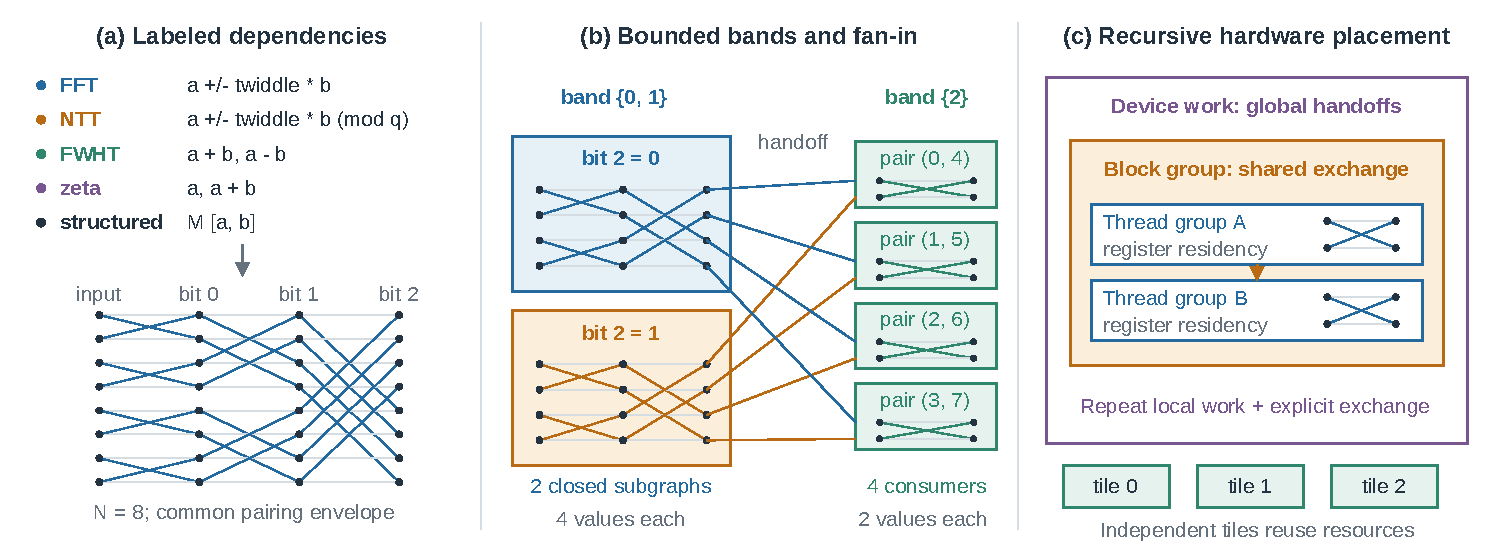
\includegraphics[width=\textwidth]{figures/drawio/exports/overview.pdf}
\caption{The organizing idea. (a) Butterfly families retain their arithmetic
labels on a common dependency construction. (b) Stage and data choices form
bounded subgraphs and explicit handoffs. (c) The construction repeats across
storage scopes, combining local residency with streamed execution. This is a
construction schematic, not a measured schedule.}
\label{fig:overview}
\end{figure*}

GPUs already provide strong arithmetic kernels and mature transform libraries
~\cite{cufft,vkfft,gpuntt,daofht}. However, a fast local core does not determine
the performance of a complete transform. Materializing every stage increases
traffic and launch overhead. Retaining more stages reduces these boundaries
but consumes registers and shared memory, potentially reducing occupancy.
A producer layout may further penalize the next consumer. These effects
couple computation, communication, and available parallel work across
transform lengths, batches, and hardware configurations. This makes the
problem more than selecting a faster pair operation. A library must decide
which dependencies to keep local and how to expose the remaining work without
turning each combination of operator, size, and device into a separate design.

Prior systems address important parts of this problem. SPIRAL and FFTX
unify transform descriptions and implementation generation
~\cite{spiral2005,fftx2018}. FlashFFTConv organizes FFT convolution around
tensor cores~\cite{flashfftconv2024}, and Welder propagates tile reuse
through computation graphs~\cite{welder2023}. These successes suggest that
the missing link is not an absence of tiling or search, but a reusable account
of which local regions and exchanges the butterfly dependencies permit.
Our question is more specific.
\textbf{Can butterfly dependencies define a reusable execution paradigm,
including both local work and the communication between local units?}
Section~\ref{sec:related} compares the organizing objects and scope of these
approaches.

We derive the execution unit from stage bits. Holding other index bits fixed
produces a \textbf{dependency-closed subgraph}, within which the selected
stages require no external values. Intersections between adjacent subgraphs
identify communication and readiness without expanding every scalar edge.
Arithmetic labels remain attached to the operations, allowing this construction
to serve FFT, NTT, FWHT, zeta, and structured stages without conflating their
semantics.

This construction supports \textbf{hierarchical hybrid dataflow}. At each
scope, stage and data positions can occupy spatial resources or reuse them
over time. A bounded subgraph retains intermediate values while independent
work streams through the resources. Repeating this choice across storage
scopes expresses workloads beyond any fixed local capacity. At a boundary,
\textbf{successor-aligned writeback} maps logical values to the consumer's
representation, potentially removing a separate reordering pass.

Our contributions are three linked pieces:
\begin{enumerate}
\item We define a \textbf{unified execution construction} from labeled
butterfly dependencies. Operator semantics, workload domains, and hardware
capabilities remain separate inputs to a joint mapping problem.
\item We define \textbf{hierarchical hybrid dataflow} through bounded
subgraph closure, residency, explicit communication, readiness, and
successor-aligned writeback. The construction scales by repeating the same
rules across storage scopes.
\item We realize and evaluate the construction with compatible cores, measured
services, bounded search, fixed-core controls, and profiler evidence. The
evaluation reports both gains and contracts where application integration is
still incomplete.
\end{enumerate}

\system{} realizes the method through block-level and resident subgraph
execution. It binds compatible cores, generates layouts and schedules, and
selects checked implementations under a finite budget. Our evaluation connects
library comparisons to fixed-core controls and trace diagnostics. The bounded
A100 80GB screen measures FFT geometric-mean latency ratios of 1.103$\times$
and 1.353$\times$ over cuFFT for its FP32 and FP64 requests, with separate
NTT and FWHT gains under their stated contracts. More directly,
changing organization improves both tested FFT cores by about 1.22$\times$.
These controls test whether the shared execution method contributes beyond
the arithmetic core itself. We first develop the organization problem from
the shared graph and prior approaches, then derive the method and its GPU
realization. The evaluation follows the same chain from overall efficiency
to the mechanisms and limits behind it.

\section{Background and Motivation}
\label{sec:background}
The organization question begins with the dependency graph. We first identify
its recurring structure and numerical variants, then use measured and analytical
examples to derive the requirements for a common method.

\subsection{Butterfly computation and its variants}
A butterfly computation combines small groups of values through a sequence
of stages. In a radix-two stage, disjoint pairs can execute independently,
but the next stage pairs their outputs differently. These changing partners
are what make local computation easy to parallelize and the complete
computation difficult to organize.
For $N=2^L$, the graph has $L$ stages and $N/2$ pair
updates per stage. A stage associated with bit $q$ pairs indices $i$ and
$i\mathbin{\oplus}2^q$. The stage sequence defines the dependency envelope,
while the pair function supplies arithmetic and coefficients. Batch instances
add independent copies of the graph. \textbf{Shared structure does not imply
interchangeable semantics.}

The family includes complex FFT, finite-field NTT, sum-and-difference FWHT,
subset and superset zeta transforms, and products of structured $2\times2$
stages. One-sided zeta updates use a subset of the full pairing dependencies.
For example, an FFT pair multiplies by a complex twiddle, an NTT pair performs
modular arithmetic, and an FWHT pair uses only sums and differences. A common
organization must retain these distinctions rather than replace every pair
with one arithmetic implementation. Multidimensional separable transforms
compose axis transforms with a shared tensor layout, making inter-axis
placement part of the same execution problem.

Cooley--Tukey (CT) and Gentleman--Sande (GS) illustrate another distinction
~\cite{cooley1965,gentleman1966}. Their local forms place twiddle
multiplication on opposite sides of addition and subtraction. Forward and
inverse computation also change coefficients, stage order, permutations, and
normalization. Stockham algorithms distribute permutations across passes
~\cite{stockham1966}. Section~\ref{sec:equivalence} explains which structural
relations survive these changes.

The requested precision, direction, normalization, and input/output layout
constrain implementation choices. Internal reordering is legal only when it
preserves the request, with adaptation included in execution cost.

\textbf{The same graph admits different organizations.}
Figure~\ref{fig:organization-tradeoffs} holds the 16-point Hadamard graph
fixed. Stagewise execution exposes eight independent pairs and transfers all
values at every stage. Two-stage bands retain four values per region and halve
materialized traffic. A whole-transform band minimizes traffic but exposes
one independent region per transform. These region counts do not fix worker
counts, since workers can cooperate within a region.

\begin{figure}[t]
\centering
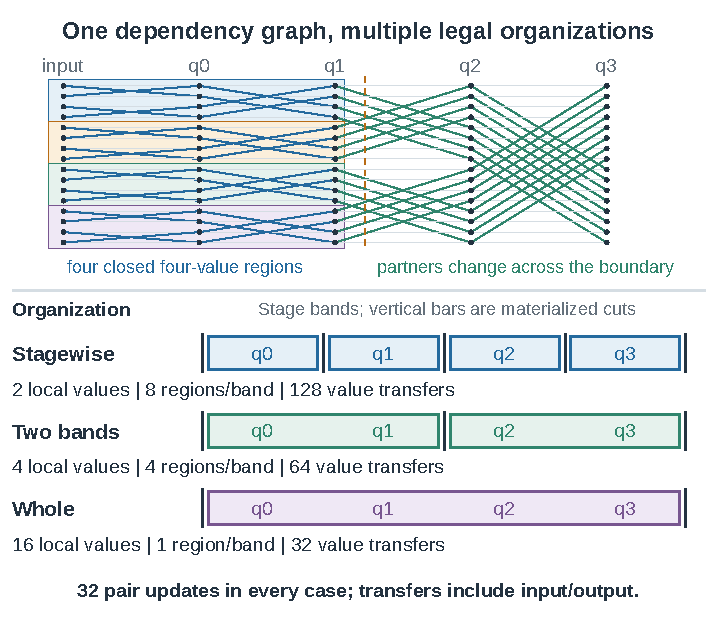
\includegraphics[width=\columnwidth]{figures/drawio/exports/organization_tradeoffs.pdf}
\caption{Grouping stages trades local state and independent regions for
fewer transfers in the same Hadamard graph. Counts are analytical.}
\label{fig:organization-tradeoffs}
\end{figure}

Storage scopes give these logical choices physical costs~\cite{ampere}.
Worker-local storage, shared storage, and external storage offer different
capacities and exchange rates. A generated codelet or imported core such as
cuFFTDx~\cite{cufftdx} must operate within those limits. The preferred grouping
therefore depends on both arithmetic service and the surrounding organization.

\subsection{The opportunity and cost of local reuse}
\label{sec:motivation}
The preceding approaches show that efficient local arithmetic and intelligent
scheduling are both available. The remaining difficulty is choosing their
boundary. How much dependent work should one local unit absorb, and how much
independent work should remain available to other units?
An \textbf{execution organization} determines which operations run together,
where values live, how producers present them to successors, and when dependent
work can begin. An arithmetic core implements a local function. Its
organization determines the communication and resources needed to compose
that function into a complete transform.

\begin{figure*}[t]
\centering
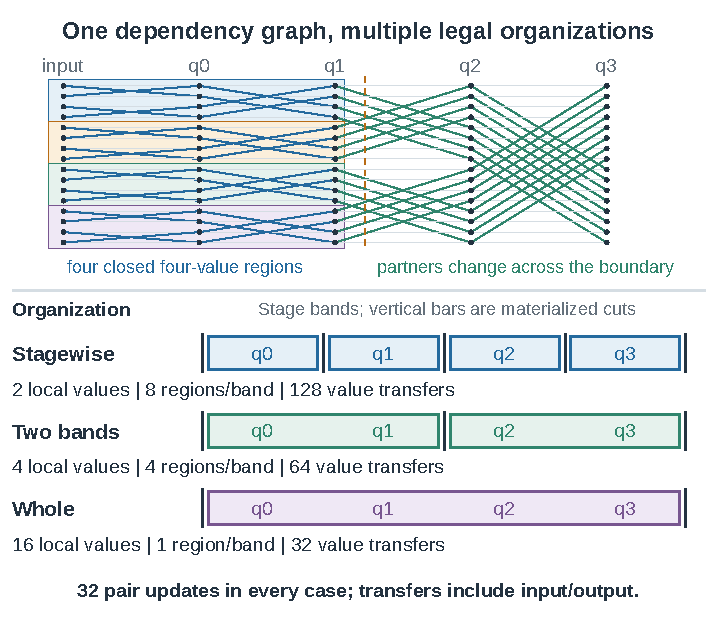
\includegraphics[width=\textwidth]{figures/drawio/exports/organization_tradeoffs.pdf}
\caption{Three organizations of the same 16-point Hadamard graph. Boxes enclose
closed components, not fixed CUDA blocks. Rows are reordered within each band
to display closure, so equal row positions across a cut need not be the same
logical value. All alternatives execute 32 pairs. Value-only reads and writes
total 128, 64, and 32 transfers per transform. Deeper bands enlarge components
and reduce their count. These analytical counts imply neither measured
speedup nor a hardware occupancy guarantee.}
\label{fig:organization-tradeoffs}
\end{figure*}

Figure~\ref{fig:organization-tradeoffs} makes the choice concrete using the
same 16-point Hadamard graph. A stage-at-a-time organization exposes eight
independent pairs but reads and writes all values at each stage. Grouping
two stages retains four values per local subgraph and halves materialized
value traffic. Retaining all four stages minimizes this traffic but leaves
only one independent whole-transform component per batch instance.
The arithmetic work is unchanged. These counts expose a trade-off rather
than a winner, because a component may itself use multiple cooperating threads
and its resource cost depends on the selected core.

The roofline opportunity follows from this distinction. For $B$ transforms of
length $N=2^L$, let $e$ be bytes per value and $G$ the number of materialized
stage groups. There are $BNL/2$ pair updates. If each group reads and writes
the array once, ideal value-only intensity is
\begin{equation}
I_{\mathrm{value}}\simeq\frac{L}{4eG}.
\label{eq:intensity}
\end{equation}
At a selected storage boundary, actual intensity is pair work divided by
transferred bytes. Its roofline ceiling is the smaller of core throughput and
bandwidth times intensity. Coefficients, transactions, cache reuse, and spills
change the traffic, while synchronization and execution efficiency determine
the distance below this ceiling.

\begin{figure}[t]
\centering
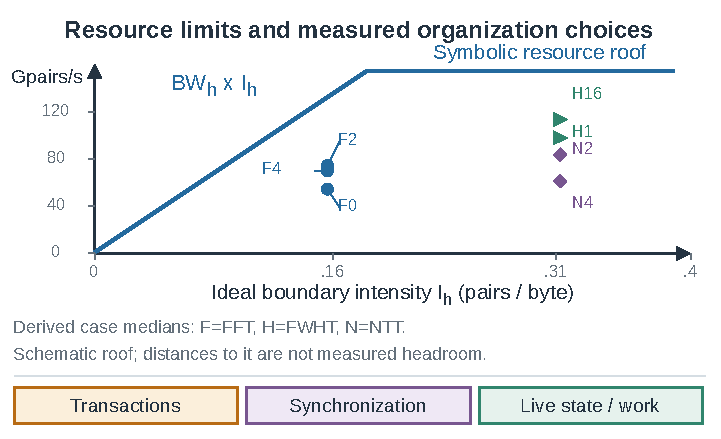
\includegraphics[width=\columnwidth]{figures/drawio/exports/roofline.pdf}
\caption{Schematic boundary roofline. Boundary intensity determines the
bandwidth ceiling, while the arithmetic core determines the compute ceiling.
Attaining either also requires sufficient ready subgraphs, resident resources,
and valid synchronization. Axes are symbolic. The lower panel states
attainment conditions, not a measured occupancy model.}
\label{fig:roofline}
\end{figure}

Reducing $G$ raises ideal intensity but enlarges live state, potentially reducing
occupancy and independent work. A faster core raises the compute ceiling
without removing a bandwidth limit. Conversely, enough arithmetic work per
byte does not ensure enough ready work to fill the machine. The ordinary
roofline identifies a resource ceiling, not a schedule that reaches it.
\textbf{The mapping must jointly choose
local reuse and enough parallel work to sustain it.}

A controlled historical V100 NTT pair illustrates the workload dependence.
At $N=2^{20}$ and batch 16, assigning two four-warp row subgraphs per CTA
instead of one improved throughput by approximately $1.154\times$ with the
same register continuation. At batch four, the change slowed execution.
The result motivates workload-dependent organization rather than a universal
preference for more local work. In particular, batch and local component size
cannot be tuned independently even when the arithmetic core is unchanged.

\subsection{Why a hierarchy and a common construction}
This trade-off suggests retaining a bounded amount of dependent computation
while exposing the remaining independent work. Stage and data positions
provide two allocation axes. A worker may execute
several stages over time, or distinct resources may serve successive stages.
Independent components may occupy different workers or reuse a worker
sequentially. Combining these choices retains a bounded region while streaming
independent work through it. We call their combination \textbf{hybrid dataflow}.
A stagewise schedule and a spatial stage pipeline are useful endpoints of
these choices, not the only organizations the framework should express.

The choice recurs across registers, cooperating threads, and groups staged
through global memory. \textbf{Hierarchy removes a fixed-capacity expression
limit.}
When a transform exceeds what a fixed number of bounded bands can express,
additional bands or recursive refinement retain the same construction.
Logical depth, materialized group count, and hardware storage levels are
therefore distinct. More levels express larger workloads but create no
additional bandwidth or storage.

More batch provides independent work to amortize startup and cover transfers.
Realizing that slack still requires lookahead, finite buffers, and available
resources. A successor needs its actual predecessor set, not merely a
contiguous prefix of producer output. The method must therefore derive both
locality and readiness from the graph.

Stage-bit dependencies provide that stable description. Changing arithmetic
alters operation labels, changing length reinstantiates the dependency domain,
and changing GPU alters feasible resources and service rates. This motivates
separate \textbf{semantics, workload, and hardware} inputs without separating
their performance effects. The separation answers a practical scaling problem.
Increasing $N$ or batch should instantiate a new work domain rather than
require a new operator implementation. Changing arithmetic should replace
compatible local functions rather than rederive the surrounding dependencies.
Changing GPU should alter feasible mappings and service costs rather than
the mathematical request.

These observations give the method three obligations. It must derive a legal
local unit, connect such units without losing dependencies or value identity,
and repeat the organization when a workload exceeds one storage scope.
The next section develops those rules. Block-level and resident subgraph
execution then provide their concrete GPU realization.

\section{Hierarchical Hybrid Dataflow}
\label{sec:method}
The motivation leaves a central question unanswered. A useful local unit
must contain enough dependent work to reuse values, yet remain small enough
to admit a feasible mapping. Choosing a tile from its size alone does not
establish that its inputs are available or that its outputs can feed the next
tile. We therefore start with the dependencies and derive the execution units
before assigning resources to them.

The construction takes an \textbf{operator contract}
covering arithmetic, coefficients, direction, normalization, and logical
ordering, a \textbf{workload domain} covering shape, batch, placement, and
strides, and \textbf{hardware capabilities} covering resources and cores.
They specialize one construction rather than independent implementations.
We first derive closed subgraphs, then compose them across storage scopes,
and finally derive their communication and the conditions for reusing the
construction across variants. The 16-point Hadamard example introduced in
the motivation serves as a concrete instance throughout.

\subsection{Dependency-closed subgraphs}
Local reuse is possible only when a chosen group contains the values needed
by all of its internal operations. The stage-bit representation makes this
condition constructive rather than a property checked after arbitrary tiling.
\textbf{A stage band determines its local data domain.}
For a radix-two transform, choose a consecutive stage band and let $Q$
contain its pairing bits. Holding every other index bit fixed gives
\begin{equation}
\mathcal I(a,Q)=\{i\mid i\text{ agrees with }a\text{ outside }Q\}.
\label{eq:component}
\end{equation}
Every pair update in the band changes only a bit in $Q$ and thus stays inside
this component. Assignments to the fixed bits partition the array into
independent components of $2^{|Q|}$ values. The band's computation on one
component is a \textbf{dependency-closed subgraph}. Closure is local to the
band, whose inputs and outputs still connect to other bands.

Any ordered stage partition defines such components. Band width controls local
reuse, while the number of components assigned to a worker controls worker
reuse. Arithmetic labels remain attached to the operations. In particular,
an FFT band may require global-index-dependent twiddles, so a standalone
smaller FFT is not automatically a compatible core.

\noindent\textbf{A running example.}
For a 16-point unnormalized Hadamard transform with stage bits $(0,1,2,3)$,
write $i=4r+c$. Two equal bands give four row subgraphs varying $c$, then
four column subgraphs varying $r$. Each uses a four-point Hadamard core.
This instantiates the two-band case in
Figure~\ref{fig:organization-tradeoffs}. The component boundary follows
which bits vary, not whether the values happen to be contiguous in the
original array. The implementation can therefore choose a representation
that matches its store and read constraints without changing the logical
computation.

\begin{figure}[t]
\centering
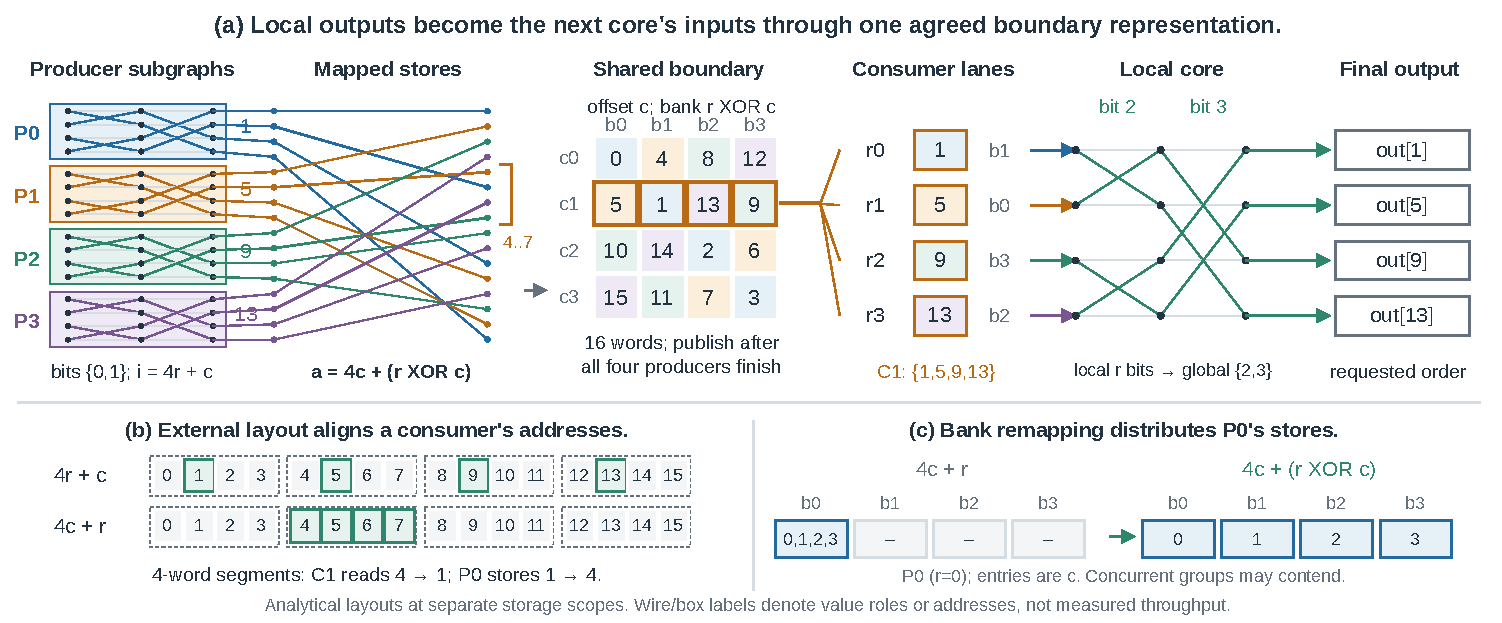
\includegraphics[width=\columnwidth]{figures/drawio/exports/hierarchy.pdf}
\caption{The 16-point Hadamard construction. Each column consumer needs one
value from every row producer. Successor-aligned writeback makes a consumer's
values contiguous. The lower panel shows refinement when local capacity limits
band width. Sizes are illustrative.}
\label{fig:hierarchy}
\end{figure}

\subsection{Hierarchical spatial and temporal choices}
\label{sec:scaling}
Closure provides an independent unit of work, but does not prescribe a
thread block, kernel launch, or fixed number of pipeline stages. Keeping
these choices open is necessary because the same subgraph can fit different
storage scopes on different targets.
\textbf{Hierarchical hybrid dataflow assigns spatial resources and temporal
reuse to both stages and data.} Successive stages can reuse a worker or occupy
different resources. Independent components can execute concurrently or stream
through the same worker. A selected region retains intermediate values while
its surrounding execution supplies independent work. The construction repeats
inside that region and across storage scopes.

A thread can retain a small subgraph in registers, cooperating threads can use
shared memory, and larger regions can use global handoffs. Refining a parent
does not require its entire intermediate array to fit on chip. Hierarchical
spatial and temporal mapping has precedents~\cite{timeloop2019}. Here,
butterfly closure and intersections determine the legal regions and handoffs.

At storage scope $h$, residency requires
\begin{equation}
\max_t\bigl(\mathrm{live}_h(t)+\mathrm{aux}_h(t)\bigr)\leq C_h,
\label{eq:capacity}
\end{equation}
where live values, coefficients, and buffers are counted in bytes. Compiled
register allocation and storage granularity further constrain the mapping.
A region that does not fit can be refined, rescheduled, or materialized at a
larger scope. \textbf{Value residency differs from worker persistence.}
A finite kernel may keep intermediates local, whereas a persistent worker may
exchange them through global buffers.

\subsection{Communication and readiness}
Local independence ends at a stage-band boundary, where pair partners change.
The next step is therefore to recover the dependencies between the units just
constructed. The same index sets that established closure also supply this
information, so communication need not be specified separately for each
operator and workload.
Adjacent components communicate through their index-set intersections.
A producer and consumer with variable-bit sets $P$ and $Q$ share values when
they agree on all bits fixed by both. Their shared variable bits $P\cap Q$
determine each nonempty intersection. Producers covering the remaining
consumer bits $Q\setminus P$ form its predecessor set. This derives
communication without enumerating scalar edges.

Fixing the bits outside $P\cup Q$ groups connected components into a
\textbf{boundary packet}. No edge crosses packets at that boundary. Within
a packet, every producer and consumer intersect on the full pairing envelope.
For complete-component publication, a consumer must therefore await every
producer in its predecessor set. One-sided operators or finer publication
units can expose finer dependencies.

In the example, a completed row cannot release a complete column. Independent
transforms can nevertheless advance concurrently, and larger transforms may
contain multiple packets within one transform. Packet membership is derived
at each boundary, not assumed to form a fixed pipeline across the graph.
A packet is a dependency domain, not an on-chip allocation or CUDA block.
Its values can be distributed among workers and global buffers.

\subsection{Reuse across variants and dimensions}
\label{sec:equivalence}
So far the construction has used one ordered stage sequence. To serve an
operator library, it must also explain what can be reused when that sequence,
its arithmetic, or its tensor interpretation changes. The reusable object is
the labeled dependency relation, not the numerical output of a different
transform.
\textbf{Structural correspondence transports organizations.}
Bit reversal maps an increasing-stride pairing envelope to a decreasing-stride
one, preserving component and boundary relations. Physical layouts must still
be evaluated for the transported access pattern.

Figure~\ref{fig:semantic-transport} shows this correspondence on eight indices.
Reversing the three index bits sends adjacent pairs to stride-four pairs.
Applying the same relabeling to every stage transports the complete envelope
and its closed regions. It does not permit stages with different arithmetic
labels to be exchanged arbitrarily.

\begin{figure}[t]
\centering
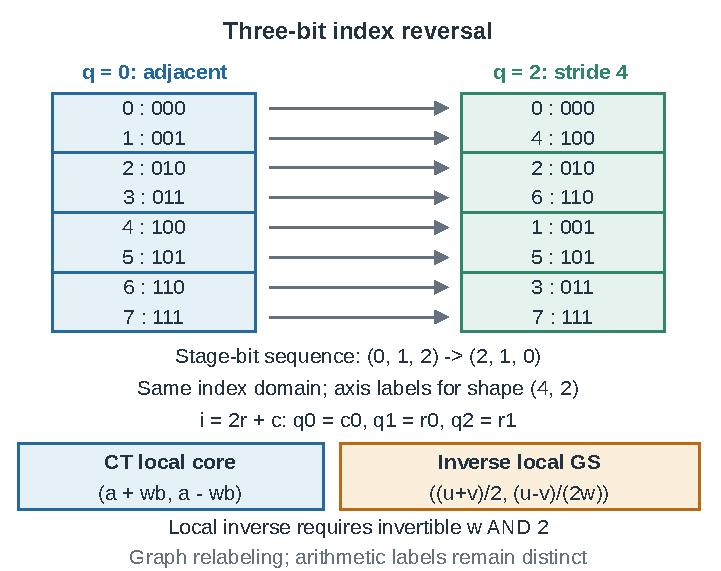
\includegraphics[width=\columnwidth]{figures/drawio/exports/semantic_transport.pdf}
\caption{Reusing the construction through explicit correspondences. Bit
reversal maps the eight-index pairing envelope and its stage-bit sequence.
Axis labels describe the same index domain for a $4\times2$ tensor.
The core inset shows a CT pair and its local inverse GS form, requiring
invertible $w$ and $2$. These are algebraic examples, not claims of identical
floating rounding, arbitrary stage commutation, or equal execution cost.}
\label{fig:semantic-transport}
\end{figure}

Arithmetic labels move separately. A CT pair computes $(a+wb,a-wb)$ and
a GS pair computes $(a+b,w(a-b))$. A GS pair with reciprocal twiddle and
one-half scaling inverts the CT pair where those inverses exist. A full
inverse also reverses stage order and applies the corresponding permutations.
Hadamard changes the local labels to sums and differences, zeta/M\"obius
exchanges one-sided addition and subtraction, and structured stages require
invertible local matrices for inversion. Numerical contracts remain explicit.

For separable power-of-two tensor axes, pairing bits can be labeled by axis
and position. Axis-stage composition then uses the same closure and boundary
rules on the tensor index domain. Axis order and inter-axis layout become
mapping choices subject to the operator's factorization. This describes a
shared construction, not a claim that every multidimensional or arithmetic
variant already has an efficient lowering.

\subsection{Correct composition}
The preceding rules separate the questions of what is computed, where each
value is placed, and when its consumer may run. Their composition must still
implement the requested complete operator.
A composed execution is correct when it covers each required operation once,
each core implements its labels, every handoff preserves value identity, and
every read occurs after production and before storage reuse. A topological
induction suffices. Correct predecessor values reach the next operation through
consistent layouts and valid lifetimes, and its arithmetic produces the
required outputs. Thus local arithmetic, boundary layout, and scheduling
carry distinct correctness obligations. The next section realizes these
obligations with block-level and resident subgraph execution.

\section{Realizing the Method with Subgraph Execution}
\label{sec:execution}
The dependency construction specifies legal work and communication but leaves
their physical implementation open. This distinction lets the same method
use a register codelet, a cooperating warp, or a block-local core without
making any one of them part of the mathematical definition. A realization
binds each dependency-closed subgraph to a core, storage scope,
and schedule. The core implements its stage bits, arithmetic, and coefficient
rules while declaring value ownership and local synchronization. Register
codelets, warp cooperation, block-local kernels, and imported components can
satisfy this contract with different resource costs.

The interface must describe more than the number of input values. A core
also declares their logical roles, which threads own them, and the
synchronization required before its outputs are visible. These requirements
connect the core to the surrounding layout and schedule. Replacing a core
can change the best organization even when the two compute the same function,
because their registers, shared storage, and exchange patterns differ.

\subsection{Successor-aligned writeback}
The first physical problem appears when a locally efficient producer leaves
its outputs in an inconvenient representation for its consumer. An explicit
permutation is always a possible implementation, but adds a pass over the
boundary data. Instead, the producer can incorporate the required placement
into its writeback when its ownership and store pattern permit it.
A producer's output representation must agree with the successor's input
representation for each logical value $i$,
\begin{equation}
\lambda_{\mathrm{out}}(i)=\lambda_{\mathrm{in}}(i).
\label{eq:handoff}
\end{equation}
Together with compatible ownership and publication, this is the
\textbf{successor-aligned writeback} rule. It can remove a separate
permutation by placing values for their next use.

One construction moves the successor's variable stage bits into low-order
address positions, placing its component in a contiguous range. In the
Hadamard example, a producer can write logical index $4r+c$ at address
$4c+r$, so the next band reads a column contiguously. Identity placement and
explicit permutation remain alternatives. Consumer locality alone does not
guarantee efficient stores, so the candidate cost includes both transactions
and any staging.

Shared storage adds a bank constraint. For an illustrative square tile with
power-of-two side $P$, $P$ banks, and one word per value, consider
\begin{equation}
\lambda(r,c)=P\,r+(c\mathbin{\oplus}r).
\label{eq:swizzle}
\end{equation}
XOR by a fixed row is a permutation. Under the single-word access pattern in
Figure~\ref{fig:banklayout}, both a row and a column reach distinct banks.
Vector values and partial warps require their actual transaction analysis.
Global layouts obey the same value-identity rule but are evaluated for
alignment, transaction width, and coalescing.

\begin{figure}[t]
\centering
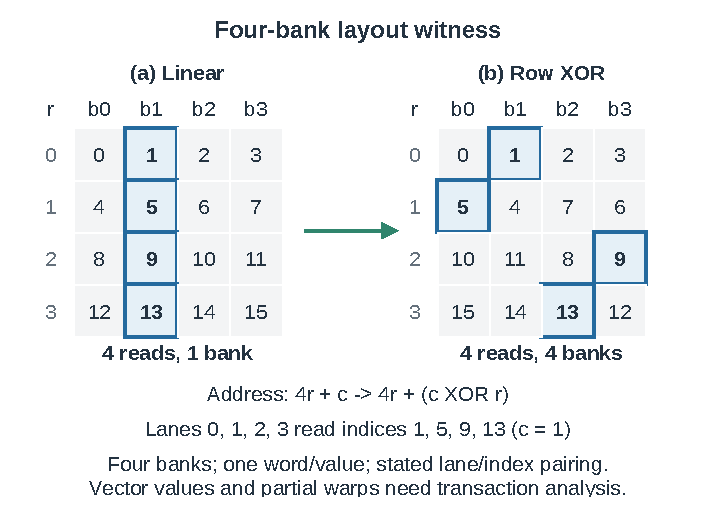
\includegraphics[width=\columnwidth]{figures/drawio/exports/bank_layout.pdf}
\caption{A four-bank layout witness. A row-dependent XOR offset distributes
a logical column across banks for the stated single-word access pattern.}
\label{fig:banklayout}
\end{figure}

\subsection{Residency, publication, and finite buffers}
Correct placement alone does not make a value ready. The row/column example
requires contributions from several producers, and reusing a buffer too early
would overwrite data still needed by a consumer. Execution therefore tracks
availability and lifetime at the same dependency granularity as the handoff.
A resident group tracks its live values and unfinished consumers. A
materialized boundary publishes a dependency unit, and the successor starts
only when its predecessor set is ready. A buffer slot is acquired before
writing, published after production, and released after the last required read.
The slot count trades lookahead against live state and synchronization cost.
Tail tiles retain their actual shape and release event.

Figure~\ref{fig:pipeline} illustrates the distinction with independent
Hadamard transforms. Completing one row leaves every column waiting for
three other rows. After the full row band publishes, its column consumers
can overlap the row work of another transform if resources permit. The
buffer holding the first transform becomes reusable only after its final
consumer read, not simply when its producer has finished.

These rules support bulk execution and pipelines across storage scopes.
Independent transforms may interleave, while a row-to-column boundary within
one transform retains its fan-in constraint. Larger batch supplies scheduling
opportunities, but legal overlap still depends on readiness, resource
availability, and buffer lifetimes.

\subsection{Composing physical services}
Once placement and lifetime are fixed, the remaining performance question is
how the local work composes. Summing isolated core times misses startup and
boundary work, while assuming ideal overlap ignores readiness and contention.
We use the actual physical groups and release rules to distinguish these costs.
For a selected physical group, a \textbf{service model} separates startup,
repeated work, and the tail,
\begin{equation}
T_{\mathrm{group}}=T_{\mathrm{start}}+R\,T_{\mathrm{step}}+T_{\mathrm{tail}}.
\label{eq:serial}
\end{equation}
The terms depend on the core, tile shape, layout, launch geometry, and storage
scope. A complete-kernel measurement already includes its launch and tail.
Bulk execution sums group services plus boundary costs not already included.

For $K$ tiles in a repeatable pipeline, the corresponding view is
\begin{equation}
T_{\mathrm{pipe}}\mathrel{\approx}T_{\mathrm{fill}}+(K-1)\,\mathrm{interval}
                  +T_{\mathrm{drain}}.
\label{eq:pipeline}
\end{equation}
Ready dependencies, finite-buffer reuse, and shared execution or memory
resources limit the interval. Overlapped groups need not retain their isolated
service rates. More independent work amortizes fill and drain and can cover
transfer latency, but cannot exceed a saturated resource's throughput.
The model ranks realizations under these assumptions rather than proving
optimality.

\begin{figure}[t]
\centering
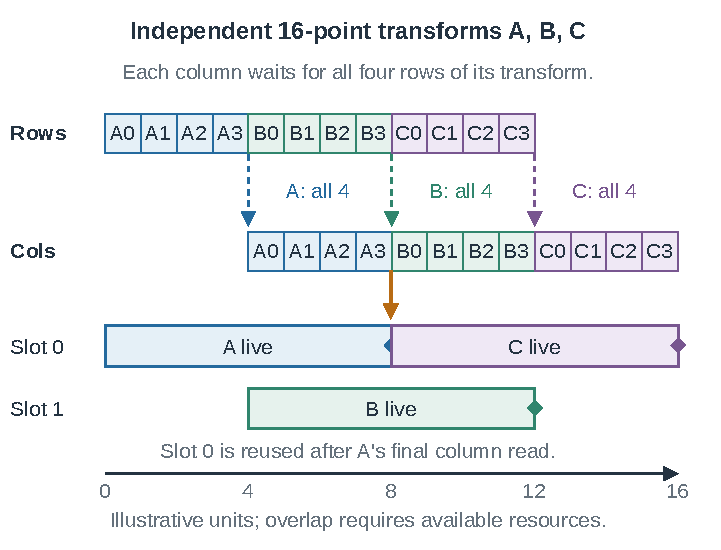
\includegraphics[width=\columnwidth]{figures/drawio/exports/pipeline.pdf}
\caption{Readiness and lifetime for independent 16-point Hadamard transforms
A, B, and C. Each column requires all four rows of its transform. Slot 0
becomes reusable by C only after A's final column read. Equal operation
durations are illustrative, not measured. Lanes denote logical work, and
cross-transform overlap requires available resources.}
\label{fig:pipeline}
\end{figure}

\section{Kernel Generation and Selection}
\label{sec:search}
Generation and selection turn the legal organizations into reusable plans.
Figure~\ref{fig:framework} follows Figure~\ref{fig:overview}'s inputs to
residency, layouts, concurrency, and handoffs.
The complete device path defines warm execution; preparation, including
compilation, is excluded.

\begin{figure}[t]
\centering
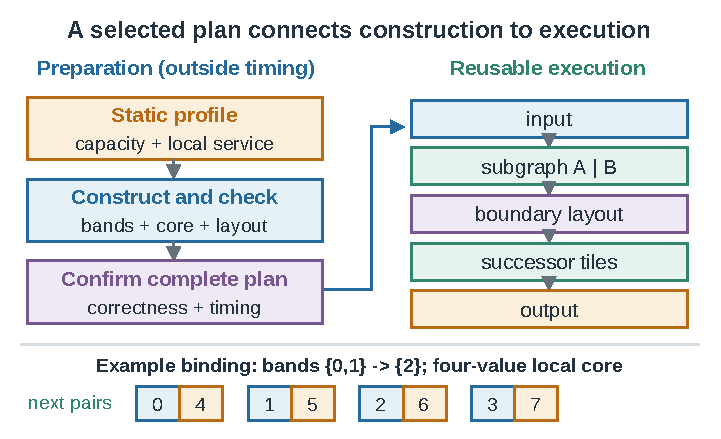
\includegraphics[width=\columnwidth]{figures/drawio/exports/system_architecture.pdf}
\caption{Preparation constructs and checks subgraph plans, then the selected
plan controls local execution and boundary exchange.}
\label{fig:framework}
\end{figure}

\noindent\textbf{Compatible realizations.}
Generation combines bands, regions, cores, storage, layouts, and bulk/pipelined
schedules while preserving arithmetic, precision, direction, normalization,
order, shape, and placement. Adaptation
costs remain included; missing compatible lowering remains a gap. Static
checks enforce dependencies and capacity; compilation exposes local allocation,
intermediate and temporary storage, and launch requirements. Numerical checks precede timing.
Failed checks remain recorded but untimed. Cache reuse requires matching
semantic, workload, hardware, and compilation assumptions.

\noindent\textbf{Service estimates.}
Services are keyed by arithmetic, core, tile shape, layout, and resource regime,
separating full and remainder tiles when necessary. Piecewise linear
interpolation stays within compatible measured regimes; missing coverage
requires measurement or an explicit gap. Composition respects predecessors,
buffers, and shared-resource contention: shared execution and memory capacity
can lengthen concurrent service intervals. Submission costs are added only when
absent from measured services. Estimates guide preparation; search instantiates
the resource characterization rather than constituting a contribution.

\noindent\textbf{Bounded selection and confirmation.}
Finite-budget selection uses bounded enumeration or model-guided exploration;
explicit evolutionary tuning adds multistart neighborhood mutation.
Multidimensional selection measures whole candidates before refining axes.
Compatible caches and calibration avoid repeated preparation. All modes share
semantic/resource constraints and retain complete organization costs.
Complete-plan timing confirms selection, separately from static ranking.
Organization comparisons distinguish explicit interventions from searched plans,
retaining actual mappings, tuning conditions, and confirmation protocols.
Finite search does not establish global optimality.

\section{Evaluation}
\label{sec:evaluation}
\subsection{Questions and experimental scope}
The central claim is that one dependency-based organization method can adapt
to different butterfly computations. It does not require every optional
mechanism to help every workload. We therefore separate five questions.
Do automatically selected plans compete with specialized libraries?
When do individual mechanisms help, and can selection avoid their costs?
Does changing organization improve a fixed arithmetic core, including after
that core is replaced? How effectively does bounded search select plans?
Finally, do operator gains survive complete application execution?
External-library comparisons establish competitiveness on their sampled
workloads. Fixed-core controls separately test whether organization causes
a gain. Neither matching a closed-source library nor losing to it alone
isolates the contribution of hierarchical hybrid dataflow.

\textbf{Matched semantics.} Each operator row specifies arithmetic and
accumulation precision, direction, normalization, input/output order, shape,
batch, placement, and strides. Required conversions are timed and adapted
paths are identified. Integer comparisons require exact agreement. Current
floating-point records retain error distributions and reference-library
errors without an adopted acceptance threshold. Their timings are exploratory
performance observations, not completed numerical acceptance.

\textbf{Separate evidence populations.} The current screen uses a pinned
runtime on A100 80GB PCIe (SM80), CUDA 12.4, and PyTorch 2.5.1.
It contains 36 one-dimensional semantic requests across FFT, NTT, FWHT, subset
and superset zeta, and structured butterflies. A separate NTT extension
contains 12 forward/inverse requests and three process trials. We retain
older core, organization, and search experiments for their named hypotheses
and builds. Historical results are not inserted into missing current cells.
The artifact provides the unified absolute-latency table and a source ledger.
% Evidence: paper/evidence/EXPERIMENT_REUSE_20261012.json; current unified_report.

A separate October 17 review covers 66 requests, including rank-1/2/3/4/8
extensions: 29 integer requests agree exactly and all 37 floating outputs
have finite same-precision error distributions. Missing GPU comparisons and
floating acceptance remain explicit gaps. This independent build and population
supplement the evidence; they do not replace or enter the 36-plus-12 headline
statistics or the frozen figures below.

\subsection{Automatically selected operator performance}
\label{sec:rc2-results}
The screen exercises the public measured-selection path, rather than a
manually chosen resident kernel. Its timing protocol warms up ten complete
calls, captures twenty calls in a CUDA graph, and reports the median of seven
event-timed replays divided by twenty. All applicable libraries use this
protocol. Compilation, plan selection, and reference checking are excluded.
The 36-point screen has one process trial per request, whereas the NTT
extension independently repeats the selected mapping in three processes.
Replay samples are not treated as independent process trials.

\begin{figure*}[t]
\centering
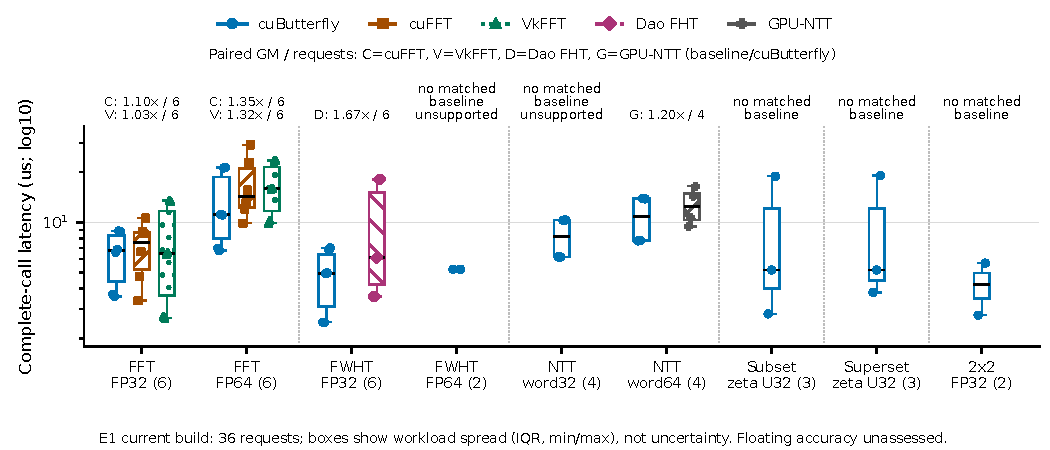
\includegraphics[width=.98\textwidth]{figures/principle_e1_latency.pdf}
\caption{Current A100 80GB operator screen. Absolute complete-GPU-call
latencies use the same graph-replay timing protocol. Each point is one
semantic request; boxes describe the sampled workload distribution, not
measurement uncertainty. Operator and precision groups remain separate.
Paired speedups are baseline latency divided by \system{} latency and are
reported separately for each competitor. Empty comparisons indicate missing
matching implementations, not wins. Floating accuracy remains under review.}
\label{fig:rc2-absolute-throughput}
\end{figure*}

Figure~\ref{fig:rc2-absolute-throughput} separates the performance of each
arithmetic family. The six FP32 FFT requests yield a geometric mean of
1.103$\times$ over cuFFT with four wins; the six FP64 requests yield
1.353$\times$ with six wins. Against VkFFT, the respective means are
1.029$\times$ and 1.325$\times$, with two and six wins.
The six FP32 FWHT requests yield 1.667$\times$ over the matched Dao interface.
These observations establish competitiveness on the sampled requests, while
preserving FFT losses rather than inferring uniform superiority from a mean.

The NTT extension crosses $N\in\{4096,65536\}$ with $B\in\{1,16,256\}$
and both directions using the same word64 field and natural-order contract.
All 12 requests pass exact checking and beat GPU-NTT, with ratios from
1.029$\times$ to 1.615$\times$ and a 1.285$\times$ geometric mean.
Its four batch-one requests are repeated controls and are not pooled with
the earlier screen. Word32 NTT, FP64 FWHT, zeta, and structured requests
retain their measured times but lack matching external comparisons here.
Thus support for these families is not itself evidence of external speedup.

\subsection{Ablation I: mechanisms and adaptive organization}
\label{sec:component-ablation}
The mechanism study asks when retaining data or overlapping work compensates
for its resource and orchestration costs. Two controls answer different
questions. A fixed-core, fixed-condition toggle explains a mechanism.
Disabling that mechanism and \emph{repeating search under the same budget}
tests its contribution to the automatically selected implementation.
Our controls include fixed-condition toggles and a newer bounded
cross-operator restricted-search study. A negative toggle result identifies
an applicability boundary, not a failure of the common representation.

For the current FFT factor-streamed control at $N=256$, $B=16384$, enabling
slice overlap changes native-core latency from 127.560 to 132.346~$\mu$s and
imported-core latency from 126.331 to 130.957~$\mu$s. Both variants still
launch three kernels, and measured L2 traffic changes by less than 0.2\%.
The imported core uses fewer registers per kernel, but its whole-call gain
is only about 1\%. These results motivate choosing overlap from its complete
cost, rather than always enabling it or treating lower register count as
sufficient evidence of higher throughput.

The October 17 selector study repeats search with stage overlap, resident
fusion, or successor layout disabled, using eight scheduled candidates per
space for FFT ($N=16384,B=16$), FWHT and NTT ($N=16384,B=4$).
FFT and FWHT timing differences are small; NTT restricted-search regret is
0.7\% for resident fusion and 2.9\% for successor layout, with overlap within
measurement noise. The latter NTT pair accepts eight restricted candidates
versus six unrestricted candidates because two unrestricted mappings fail
legality checks. These traces establish an executable restriction protocol
and its candidate-population effects, not a stable universal mechanism gain;
independent winner confirmation and broader requests remain necessary.

\begin{table}[t]
\centering\small
\caption{Current FFT core/overlap diagnostic. Ordinary latency is the median
of three process trials; counters are from separate NCU kernel captures.
Registers list the three kernels in execution order. L2 totals are decimal
MB, not an average bandwidth or a complete application traffic estimate.}
\label{tab:component-counters}
\begin{tabular}{@{}llrrl@{}}
\toprule
Core & Overlap & $\mu$s & L2 MB & Registers\\\midrule
Native & Off & 127.560 & 201.83 & 61/61/63\\
Native & On & 132.346 & 201.57 & 61/61/63\\
Imported & Off & 126.331 & 201.48 & 52/52/36\\
Imported & On & 130.957 & 201.54 & 52/52/36\\
\bottomrule
\end{tabular}
\end{table}

The earlier layout/depth and batch controls reach the same qualitative
conclusion. Writer-aligned layout loses in its three tested pairs, while
greater resident depth wins in three pairs. Pipeline batching loses to bulk
in 27/27 A100 80GB comparisons. In a matched $N=4096$, $B=64$ example,
ordinary timing is 29.266~$\mu$s for bulk and 45.636~$\mu$s for the pipeline.
Nsight Systems observes overlap, but the pipeline issues eight launches per
call instead of two. The limitation is the balance between useful overlap
and fragmentation, not whether overlap can be expressed.

\textbf{Counter boundaries.} NCU counters describe sampled kernels;
ordinary timing measures performance. Copies are listed separately. For
example, the fixed-mapping Dao FWHT diagnostic contains a 2~MiB device copy
outside its NCU kernel byte totals. We do not interpret those totals as
complete-call traffic. The deliberately underfilled stagewise diagnostics
are likewise excluded from claims about a well-tuned baseline. The artifact
retains their registers, shared-memory conflicts, traffic, and wait metrics.

A separate current-build six-request control changes stage partitioning for
FFT, FWHT, and word64 NTT at $N=4096,B=4$ and $N=262144,B=1$.
Stagewise-over-resident-8 ratios range from 10.87$\times$ to 22.44$\times$.
The paired FWHT profile records 18 versus three kernels at the larger shape.
These large ratios expose the launch and global-boundary cost of the
stagewise control, not an optimized external-library comparison.

\subsection{Ablation II: organization benefits at fixed core}
\label{sec:core-organization}
Whole-library improvements could otherwise be explained by a larger
collection of arithmetic kernels. To isolate organization, we reuse a
four-cell experiment that embeds the same 16-point arithmetic leaf in two
execution organizations, then repeats the comparison with another leaf.
The core axis selects native register arithmetic or cuFFTDx Thread.
The organization axis selects stagewise HBM exchange or a resident two-stage
prefix; later stages retain the same global-stage template.

\begin{figure}[t]
\centering
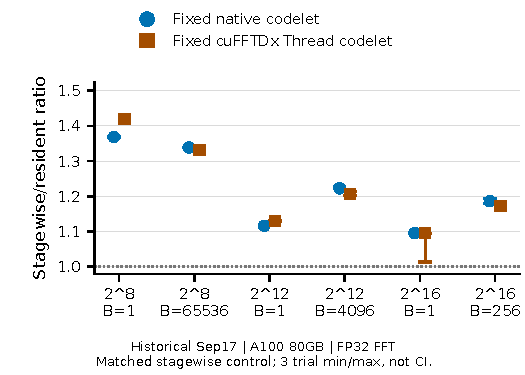
\includegraphics[width=\columnwidth]{figures/principle_core_organization.pdf}
\caption{Historical A100 80GB fixed-leaf organization control. Each series
keeps its arithmetic leaf fixed and compares stagewise-HBM with
resident-prefix-2 execution. Six workloads cross three lengths with latency
and throughput batches. Ratios use three-trial median latencies; error bars
show paired trial ranges, not confidence intervals. Values above one favor
residency. Both leaf implementations benefit. This independent
mechanism executable is distinct from the current public-library cohort.}
\label{fig:core-organization}
\end{figure}

Six FP32 workloads each have four cells and three trials, producing 72 rows.
Each trial uses complete-batch reference checks, 10,000 warmups, and 100
repetitions. Residency improves all six workloads for both cores, with
geometric means of 1.217$\times$ and 1.221$\times$
(Figure~\ref{fig:core-organization}). Replacing the core at fixed organization
contributes 1.042$\times$ for stagewise and 1.046$\times$ for resident
execution. The organization benefit is therefore separately visible within
each core, rather than being attributed to core substitution.

The fixed object is the arithmetic leaf, not the entire GPU kernel.
For $N=256$, $B=1$, stagewise and resident execution launch 16 and 256
threads respectively. Shared storage, parallelism, and launch count are
part of the organization treatment; the stage-zero wrappers also differ in
source. We therefore make no claim of identical wrapper instructions or
launch geometry. A separate A100 40GB replication retains same-core
organization gains of 1.226$\times$ and 1.231$\times$; its trials are not
pooled with the 80GB results.

\textbf{Prefetch transfer across local cores.}
A newer A100 80GB FP64 control fixes $N=65536$, $B=16$, two 256-point
factor transforms, four parallel local transforms per CTA, and 16 elements
per thread. Both the repository's auditable register core and cuFFTDx Block
use the same factor execution template and writer-aligned handoff.
Only the number of tile groups consumed per CTA and the prefetch depth vary.
Figure~\ref{fig:factor-organization} reports every tested organization and
the matched complete cuFFT call.

\begin{figure}[t]
\centering
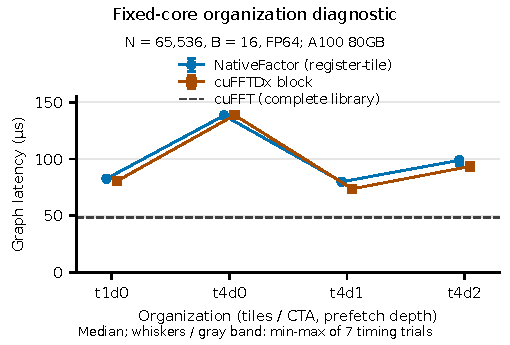
\includegraphics[width=\columnwidth]{figures/factor_organization_20261025.pdf}
\caption{Fixed-core organization diagnostic on A100 80GB, FP64,
$N=65536$, $B=16$. For example, \texttt{t4d1} denotes four consecutive
tile groups per CTA and prefetch depth one. Markers show complete-Graph median latency and whiskers
show the range of seven rounds in one process, not independent-process
confidence intervals. One-step prefetch helps both cores; deeper prefetch
regresses, and complete cuFFT remains faster.}
\label{fig:factor-organization}
\end{figure}

At four tile groups per CTA, one-step prefetch reduces native-core latency
from 138.377 to 79.974~$\mu$s and cuFFTDx latency from 138.684 to
73.762~$\mu$s, giving 1.730$\times$ and 1.880$\times$.
The faster one-tile synchronous alternative takes 82.671 and
80.657~$\mu$s, so gains against that alternative are only
1.034$\times$ and 1.093$\times$. Depth two regresses for both cores.
cuFFT takes 48.503~$\mu$s and remains faster on this request.
All outputs are finite and relative L2 errors against CPU FP64 are below
$7.4\times10^{-16}$, without introducing a numerical acceptance threshold.
This control demonstrates conditional prefetch benefits across cores.
It does not compare the full method against either core's original library
organization, establish automatic selection, or supersede the historical
leaf-residency experiment.

A historical cross-arithmetic study holds the shared-iterative arithmetic
core and physical groups fixed while changing local stage partitioning.
At $N=4096$ and batches 1/1024, FWHT improves by 1.137/1.302$\times$ and
word64 NTT by 1.073/1.091$\times$. This extends evidence for same-core
organization gains across arithmetic families. It is not a two-core factorial
for either family, nor a change to the groups' HBM boundaries. Its lowering
changes group-local shared/register exchange and synchronization.
Completing that crossing for FWHT, NTT, zeta, and structured
butterflies is a separate coverage requirement; radix labels alone do not
establish interchangeable core implementations.

New current-build controls separately compare shared-core FWHT stage
partitioning, temporal FWHT radix-2/radix-4 cores, and specialized NTT
radix-2/vector-radix-4 cores. All six rows pass their recorded correctness
checks. Their different shapes and lowering support domains do not form a
two-core/two-organization crossing, so the wider factorial gap remains.

\subsection{Coverage, selection, and preparation cost}
\label{sec:selection-evaluation}
The common interface combines semantic dimensions instead of assigning a
separate evaluation protocol to each named variant. The present screen does
not exhaust their Cartesian product. Earlier precision, inverse, layout,
and multidimensional records remain separately identified coverage evidence.
The broader historical RC2 FFT distribution reports 21/36 wins and a
1.031$\times$ geometric mean over cuFFT, and 13/20 wins with 1.026$\times$
over VkFFT. Those builds and workloads differ from the current screen;
the stronger current means are not a like-for-like version improvement.
The RC2 distribution and 27-point contiguous FFT scaling study remain
separate artifact records.
Likewise, the A100 40GB replication is a same-architecture experiment;
historical V100 results do not establish same-version cross-architecture
portability.

Selection is evaluated against the best \emph{measured} candidate, with
candidate coverage, ordering, and preparation cost reported independently.
In an earlier 16-candidate replay, informed policies find the pool best at
budgets four, eight, and sixteen. Random search's mean selected-time to
pool-best ratios are 1.486, 1.002, and 1.000 for FFT, and 2.228, 1.074,
and 1.000 for NTT. The stage-service policy has no covered priors in this
replay and falls back to structural ordering. These results support
finite-pool prioritization, not calibrated prediction accuracy, global
optimality, or online tuning cost.

Install-time service calibration and post-install tuning are implementation
stages of this selection process. Their presence does not establish that
every lowering consumes the resulting model. In the current implementation,
native multidimensional plans use complete-plan measurement and a persistent
cache separately from the rank-one calibrated registry. The application
experiment explicitly tunes those plans outside timing and requires cache
replay during measurement. Search, compilation, first use, and steady-state
execution remain separate costs. The bounded restricted-search study above
adds current cross-operator evidence; independent winner timing and online
preparation costs remain necessary for the adaptive-selection claim.

\subsection{Complete applications and batch scaling}
\label{sec:application-evaluation}
Finally, we test whether the selected organization remains useful after
integration. FFT image filtering and FNO/NeuralOperator cover image-domain
and neural spectral workloads; QuaRot/Llama covers FWHT, and HEonGPU CKKS
supplies the NTT application~\cite{neuraloperatorcode,quarotcode,heongpucode}.
All variants use identical inputs, weights or keys, and precision. The timed
boundary includes surrounding GPU work, required packing, conversions,
and synchronization. Model loading, compilation, reusable plans,
and first use are excluded and recorded separately.

\begin{figure*}[t]
\centering
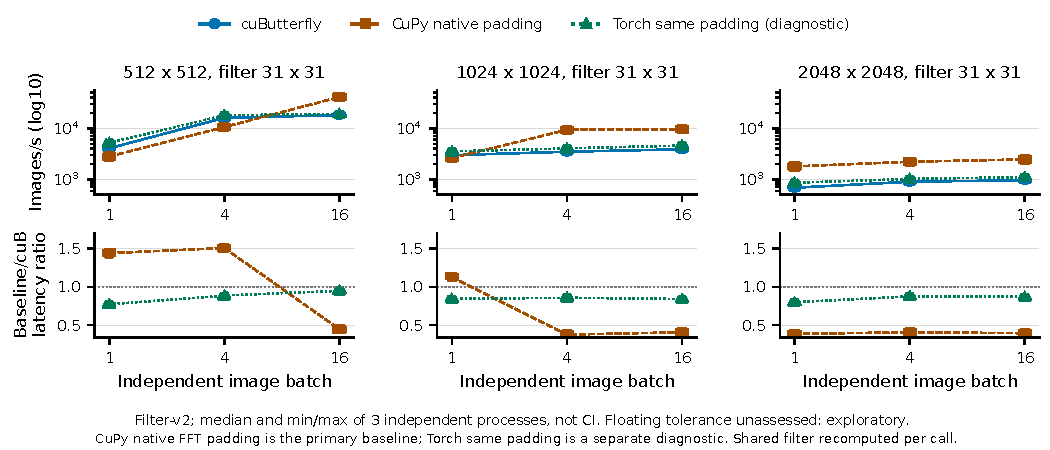
\includegraphics[width=.98\textwidth]{figures/principle_application_throughput_ratio.pdf}
\caption{Complete FP32 image-filter calls on A100 80GB, using independent
images and the same $31\times31$ filter at each batch. Each size has three
independent process trials with rotated method order. CuPy uses its native
FFT padding; the same-padding PyTorch/cuFFT path is a separate diagnostic.
All required padding, transforms, multiplication, and cropping are timed.
These are measured exploratory results, with floating error reported and
no adopted acceptance threshold. Increasing batch improves throughput but
does not guarantee a better ratio against the competitor. Error bars show
the range across three process trials, not a confidence interval.}
\label{fig:application-batch}
\end{figure*}

The filter matrix crosses image edges 512, 1024, and 2048 with batches one,
four, and sixteen. Each call recomputes one shared filter spectrum; none of
the backends uses a cached filter to gain an artificial advantage. After
untimed tuning, every \system{} plan in all three process trials replays its
persistent cache. The maximum observed relative $L_2$ error is
$5.76\times10^{-7}$ for \system{} and $3.95\times10^{-7}$ for CuPy.

Figure~\ref{fig:application-batch} preserves the unfavorable cases.
\system{} wins three of nine comparisons, including 1.448$\times$ and
1.516$\times$ for 512-edge images at batches one and four. At batch sixteen,
the same size reaches about 18,109 images/s versus CuPy's 40,812 images/s.
The larger-image cases also expose a gap. \system{} currently pads to powers
of two, whereas CuPy selects smaller supported FFT extents; the same-padding
diagnostic remains faster as well. Extra transform work is therefore one
boundary, but cannot explain the entire difference. The data do not support
claiming that more independent inputs alone eliminate integration costs.

An independent October 18 fixed-filter Graph cohort changes that contract:
all three backends cache the filter spectrum before timing and use matching
fast padding ($1080^2$ or $2100^2$), with $B=16$ and a $31^2$ filter.
For image edges 1024/2048, complete-call medians are 1.406/5.731~ms for
\system{}, 1.500/5.904~ms for CuPy, and 1.533/6.007~ms for Torch/cuFFT.
Timing includes input device copies, image padding, transforms, multiplication,
cropping, and independent output copies; setup and capture are excluded.
Changed/restored-input and output-lifetime checks pass. These five-sample,
single-process observations retain floating error reports without an adopted
acceptance threshold. They show gains for these two cached-filter requests;
the nine-point recomputed-filter cohort and its losses remain separate.

We also measure a 2D periodic spectral Poisson endpoint at $N=2048$, $B=16$,
FP32, with the same complete copy boundary for all backends. The adaptive xD
plan measures axis candidates after the budget repair and replays them through
a CUDA Graph. Figure~\ref{fig:application-poisson} shows twenty steady-state
calls in one process, not independent process trials.

\begin{figure}[t]
\centering
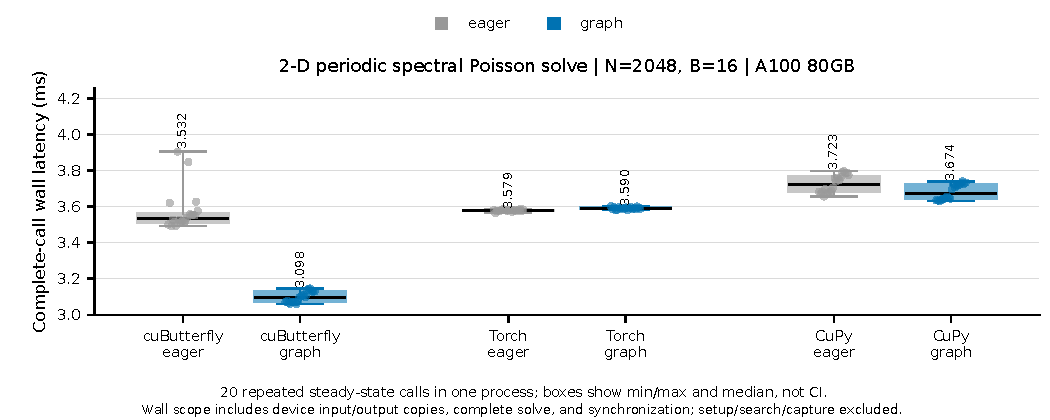
\includegraphics[width=.99\columnwidth]{figures/principle_application_poisson_endpoint.pdf}
\caption{Measured 2-D periodic spectral Poisson endpoint on an A100 80GB at
$N=2048$, $B=16$. The boundary includes device copies, both FFTs, the
frequency-domain multiplier, and synchronization; setup, search, and capture
are excluded. Boxes contain twenty steady-state calls from one process and
labels show medians.}
\label{fig:application-poisson}
\end{figure}

Graph medians are 3.098~ms for \system{}, 3.590~ms for Torch, and 3.674~ms
for CuPy, giving 1.159$\times$ and 1.186$\times$ against the two baselines.
The adaptive plan uses two fused axis launches per direction and removes the
four serialized transpose kernels and separate scale kernel of the fallback.
This measured endpoint remains separate from the nine-point image-filter cohort.

\begin{table}[t]
\centering\small
\caption{Other completed application records, kept separate from the filter
cohort. Times are milliseconds per complete call. QuaRot uses two process
trials with identical random weights; FNO uses its separately recorded
three-trial prior-day cohort. CKKS uses a separate cohort below.}
\label{tab:applications}
\begin{tabular}{@{}lrrrl@{}}
\toprule
Application & $B$ & \system{} & Baseline & Backend\\\midrule
QuaRot 512/32 & 1 & 2533.32 & 2482.87 & Dao\\
FNO $64^2$ & 4 & 2.946 & 2.783 & cuFFT\\
FNO $128^2$ & 4 & 2.965 & 2.810 & cuFFT\\
\bottomrule
\end{tabular}
\end{table}

The repaired QuaRot path reproduces the baseline outputs exactly for the
measured random-weight model, but its complete prefill-plus-decode call is
about 2\% slower (Table~\ref{tab:applications}). It uses the SDPA fallback,
not a FlashAttention comparison. FNO also remains slower. These records
measure implementation consistency and execution, not trained-model quality.
QuaRot batch expansion remains separate unfinished coverage.

The October 19 CKKS study tests whether batching corresponding NTT stages
across independent ciphertexts carries organization gains into complete
operations. It covers key switching, square/relinearize/rescale, that chain
followed by key switching, and slot rotation, at $B=1,8,32$.
All 36 configurations and 144 execution paths produce elementwise-identical
ciphertexts. Four paths share inputs and keys: native loop, \system{} loop,
native-core batch, and \system{} batch. Both batched paths share graph
organization and gather/scatter; the native batched control is constructed
by this integration, not an upstream batch API.

\begin{table}[t]
\centering\small
\caption{Independent CKKS complete-Graph cohort. Geometric mean ratios are
baseline over \system{} batch; above one favors \system{}. Each row contains
four $B=1$ and eight $B=8,32$ configurations. Loop and batch baselines remain
separate. All graph packing, NTT, writeback, and non-NTT work is timed.}
\label{tab:ckks-batch}
\begin{tabular}{@{}lrrr@{}}
\toprule
Method / $N$ & $B=1$ loop & $B>1$ loop & $B>1$ batch\\\midrule
I / 16384 & 0.723 & 1.862 & 1.124\\
I / 65536 & 0.884 & 1.195 & 1.143\\
II / 16384 & 0.723 & 1.755 & 1.128\\
\bottomrule
\end{tabular}
\end{table}

All 24 multi-ciphertext configurations beat both native controls, whereas
forced batching loses for all 12 $B=1$ configurations. Two large-$N$ rotation
cases also prefer \system{}'s own loop to its batch path. Application-level
loop/batch selection is therefore still required; these measurements do not
establish an automatic policy. Timing uses twenty rotated rounds of ten
Graph replays, with thermal guards and default dynamic clocks; setup, search,
capture, encryption, and checking are excluded. The context uses
$Q=[50,40,40]$, $P=[50]$ or $[50,50]$, scale $2^{40}$, and
\texttt{sec\_level=none}. These are complete FHE operations and short chains,
not full bootstrap or production-security validation. Request-level RNS
tuning remains distinct from installation-model integration. Thus sampled
application gains now complement the operator and organization evidence,
while broader cross-core, application, and platform coverage remains open.

\section{Related Work}
\label{sec:related}
\begin{table}[t]
\centering
\caption{Representative systems expose different organization choices.}
\label{tab:related-work}
\footnotesize
\setlength{\tabcolsep}{2pt}
\renewcommand{\arraystretch}{1.08}
\begin{tabular}{@{}>{\raggedright\arraybackslash}p{.205\columnwidth}>{\raggedright\arraybackslash}p{.14\columnwidth}>{\raggedright\arraybackslash}p{.275\columnwidth}>{\raggedright\arraybackslash}p{.32\columnwidth}@{}}
\toprule
System & Ops./\allowbreak object & Decomposition basis & Organization / resources \\
\midrule
FFTW~\cite{fftw2005} & FFT, DCT/\allowbreak DST & Recursive plans & Codelet composition; empirical planning \\
\addlinespace[2pt]
VkFFT~\cite{vkfft2023,vkfft} & FFT, DCT & Grouped strided transforms & Layout choices \\
\addlinespace[2pt]
GPU-NTT~\cite{gpuntt2023,gpuntt2025} & NTT & Merge / Four-Step & Locality; kernel count; block shape \\
\midrule
TensorIR~\cite{tensorir2023} & Tensor ops. & Block signatures & Outer transformations; tensorization \\
\addlinespace[2pt]
Welder~\cite{welder2023} & DNN graphs & Tile connections; shape propagation & Hierarchical reuse; traffic / footprint \\
\addlinespace[2pt]
Timeloop~\cite{timeloop2019} & DNN layers & Workload / mapping separation & Spatial / temporal tiling; resource costs \\
\midrule
\system{} & FFT, NTT, FWHT & Stage bits; closed regions; intersections & Stage / data reuse; live state, traffic, core / ready work \\
\bottomrule
\end{tabular}
\end{table}

Related systems optimize transform formulas, arithmetic cores, tensor programs,
and hardware mappings.

\noindent\textbf{Transform generation and specialized execution.}
FFTW combines codelets with empirical planning; SPIRAL/FFTX generates
transforms and surrounding computation from algebraic descriptions
\cite{fftw2005,spiral2005,fftx2018}. VkFFT generates GPU implementations with
grouped strided transforms and layout choices. GPU-NTT optimizes locality,
kernel count, block size, and shape
\cite{vkfft2023,vkfft,gpuntt2023,gpuntt2025}.
FlashFFTConv combines tensor-core FFT decomposition, batch/hidden tiling,
and memory-aware fusion~\cite{flashfftconv2024}. HadaCore maps FWHT chunks
to warps and vectors to threadblocks with shared-memory transposes
\cite{hadacore2024}. These systems optimize both arithmetic and organization.

Table~\ref{tab:related-work} separates their representative operators, units,
stage decompositions, independent-work mappings, and boundary mechanisms.
A GPU kernel is a launched program; a tile subgraph groups computation and
values for scheduling and residency. Kernels can execute tile subgraphs, and
larger subgraphs can span kernels. Stage fusion can retain intermediates while
reusing execution resources over time, so it does not alone establish a
spatial pipeline.

\noindent\textbf{Tensor compilation and tile scheduling.}
TVM separates computation from scheduling~\cite{tvm2018}; Ansor searches
hierarchical schedule sketches~\cite{ansor2020}; ROLLER constructs
hardware-aligned tiles~\cite{roller2022}. TensorIR provides block signatures,
outer transformations, and tensorization~\cite{tensorir2023}. Welder connects
producer/consumer tiles and schedules reuse through traffic and footprint
estimates~\cite{welder2023}. These establish tiling and reusable compute
interfaces. Their generality alone does not verify transform-specific support.
For butterflies, the changing pair relation identifies the values needed by
a stage group and the producers that a successor must await, before choosing
a physical tile or arithmetic core. This separates dependency construction
from a particular kernel implementation while preserving the operator's
arithmetic, direction, ordering, and precision contract.

\noindent\textbf{Hierarchical dataflow and positioning.}
Eyeriss analyzes data movement under controlled resources; Timeloop separates
workload, architecture, and hierarchical spatial/temporal mappings
\cite{eyeriss2016,timeloop2019}. Applying these principles to butterflies
requires legal resident tile subgraphs and their remaining communication. GPU
blocks also share resources, precluding an assumption of dedicated pipeline
hardware.

Our distinction concerns the common dependency interface. SPIRAL/FFTX derives
implementations from algebraic transform decompositions, including surrounding
computation~\cite{spiral2005,fftx2018}. Timeloop evaluates hierarchical mappings
from workload and architecture descriptions~\cite{timeloop2019}. These precedents
motivate separating arithmetic from organization; that separation alone is not
our novelty. We derive the butterfly-specific link between dependencies and
resource demand: stage-bit sets construct dependency-closed regions, and their
intersections derive communication and readiness
(Section~\ref{sec:method}). Spatial and temporal organization then determines
the demands evaluated against hardware constraints. The contribution is this butterfly-specific construction, not the general
idea of spatial/temporal dataflow or a claim that prior systems cannot express
equivalent programs. It retains specialized arithmetic across workloads and
hardware constraints. The fixed-core experiments in Section~\ref{sec:core-organization} isolate this organization
effect from arithmetic substitution.

\section{Conclusion}
\system{} derives resource demands and executable handoffs from butterfly
dependencies. Hierarchical hybrid dataflow uses this construction to organize
compatible cores and workloads under hardware constraints. Fixed-core controls
establish conditional organization gains, while library and application
comparisons measure practical benefits and losses on the tested A100 workloads
and numerical contracts. Cross-architecture performance remains unvalidated.


% The reference list is dense; keep it one step below
% body text while leaving the IEEE conference geometry and body size intact.
{\scriptsize
\bibliographystyle{IEEEtran}
\bibliography{references}
}

\end{document}
